\subsection{Distributon of the Eigentrust Scores}
	\label{eigentrust_distribution_section}
	\begin{figure}[H]
	\centering
	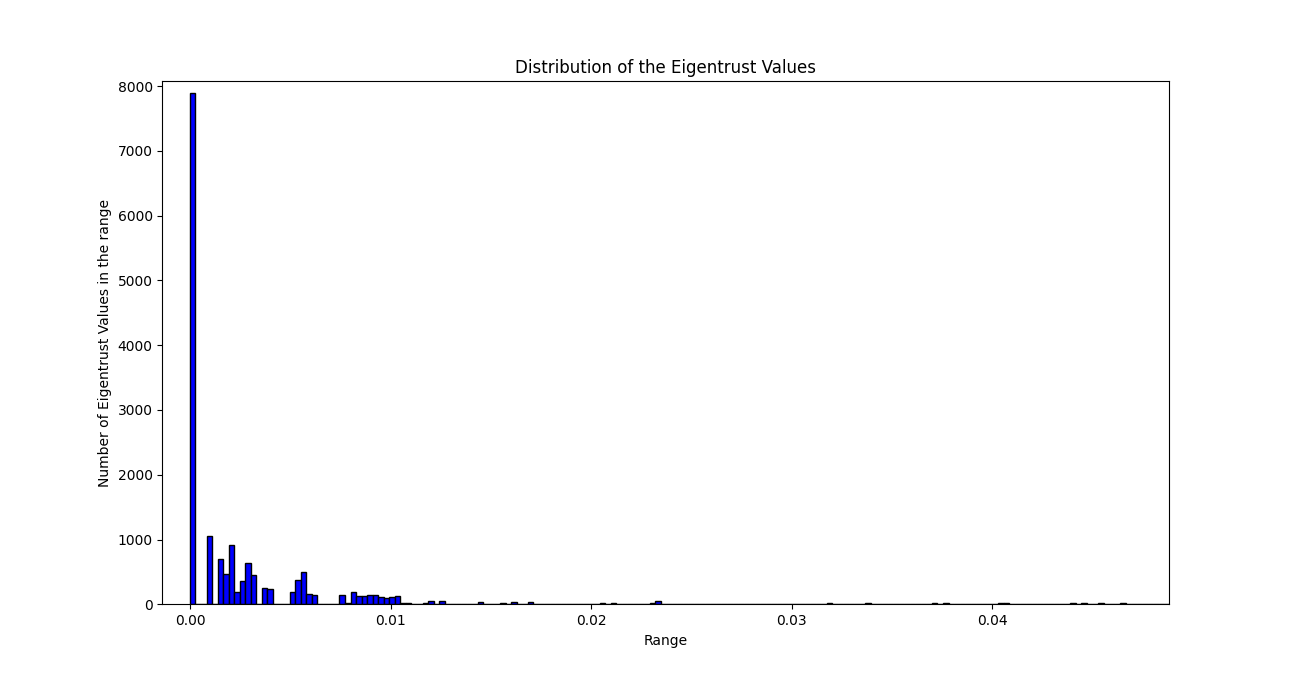
\includegraphics[scale=0.42]{eigentrust_distribution_detailed}
	\caption{Distribution of the Eigentrust scores before filtering. As can be seen, nearly 17500 of the customers have zero Eigentrust.}
	\label{fig:eigentrust_distribution_figure}
	\end{figure}
	\begin{figure}[H]
	\centering
	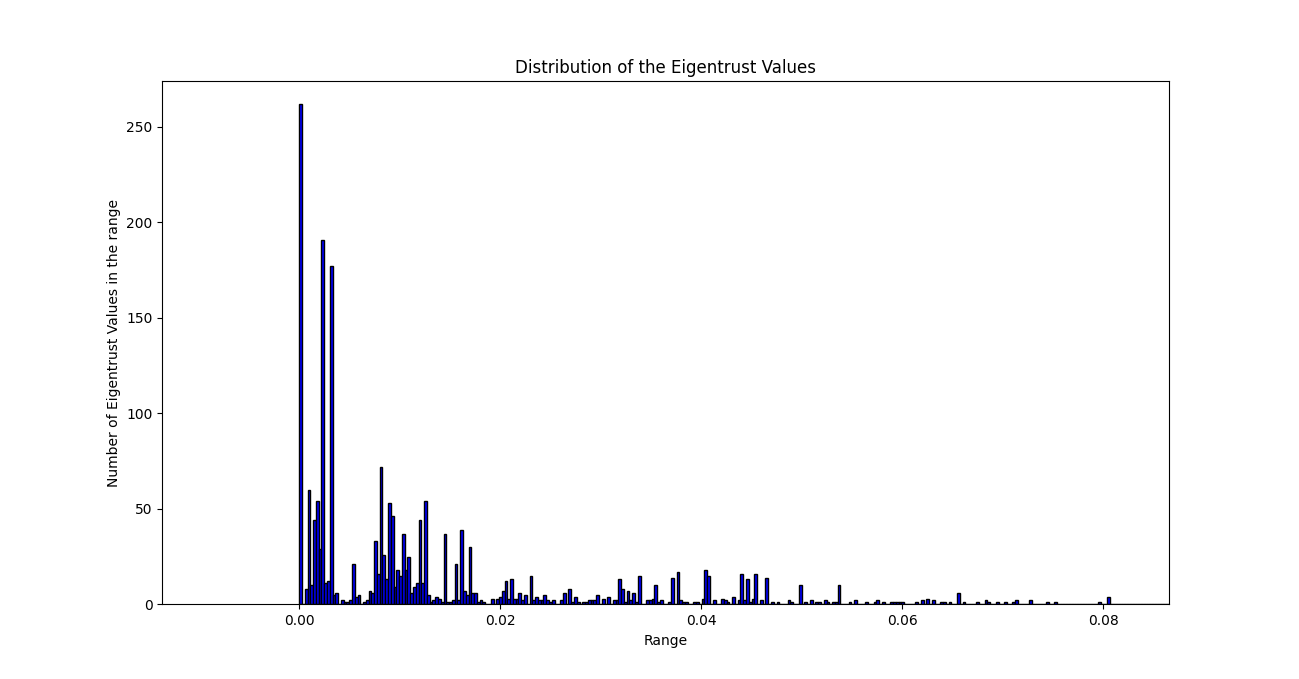
\includegraphics[scale=0.42]{eigentrust_distribution_detailed_after_filter}
	\caption{Distribution of the Eigentrust scores after filtering.}
	\label{fig:eigentrust_distribution_figure_after_filtering}
\end{figure}
\subsection{Libraries Used in Implementation Phase}
	\subsubsection{\href{https://neo4j.com/}{Neo4j}}
	Neo4j is a graph database management system where data is organized as nodes, relationships, and properties. The communication between recommender and the database is maintained by Neo4j driver.
	\subparagraph{Driver Installation}:
	\begin{lstlisting}[language=bash]
	pip install neo4j
	\end{lstlisting}
	
	\subparagraph{Configuration}:
	\begin{lstlisting}[language=python]
	import neo4j
	...
	
	uri = self._config["database"]["neo4j"]["uri"]
	user = self._config["database"]["neo4j"]["user"]
	password = self._config["database"]["neo4j"]["password"]
	
	self._driver = neo4j.Driver(uri, auth=(user, password))
	
	\end{lstlisting}
	
	\subparagraph{Sample Usage}:
	\begin{lstlisting}[language=python, caption=Neo4j driver example]
	import neo4j
	...
	
	def get_customer_trust(self, customer_id):
	
		query = (
			f"MATCH (u:Customer)-[r:BELONGS_IN]->(:Community) "
			f"WHERE u.id = {repr(customer_id)} "
			f"RETURN r.eigentrust"
		)
	
		with self._driver.session() as session:
			return tuple(session.run(query).single())
	
	\end{lstlisting}
	
	\subsubsection{\href{https://numpy.org/}{Numpy}}
	NumPy is a library for the Python programming language, adding support for large, multi-dimensional arrays and matrices. Since the core of Numpy is optimized C code, performing the calculations in the recommendation process using Numpy matrix provides serious time savings.
	\subparagraph{Installation}:
	\begin{lstlisting}[language=bash]
	pip install numpy
	\end{lstlisting}
	
	\subparagraph{Sample Usage}:
	\begin{lstlisting}[language=python, caption=Numpy example]
	import numpy as np
	
	class TrustBasedFilterer(object):
	...
	
		def _create_customers_versus_products_table(self):
	
			self._customers_versus_products_table = np.zeros(
				(self._unique_customers.shape[0],
				self._unique_products.shape[0]),
				dtype=np.bool,
				)
	
			self._customers_versus_products_table[
				self._sales[:, 0],
				self._sales[:, 1],
			] = True
	\end{lstlisting}
	
	\subsubsection{\href{https://www.scipy.org/}{Scipy}}
	SciPy is a Python library used for scientific computing. Similar to Numpy, many of the Scipy functions are written in C which provides a solution to the slowness caused by interpretation. For this reason, we prefer to use the "Dijkstra's Algorithm" provided by Scipy rather than implementing it by ourselves.
	\subparagraph{Installation}:
	\begin{lstlisting}[language=bash]
	pip install scipy
	\end{lstlisting}
	
	\subparagraph{Sample Usage}:
	\begin{lstlisting}[language=python, caption=Scipy example]
	from scipy.sparse import csr_matrix
	from scipy.sparse.csgraph import dijkstra
	
	class Graph(object):
	...
	
		def _create_distance_matrix(self):
	
			self._create_adjacency_matrix()
	
			self._adjacency_matrix = \
				csr_matrix(self._adjacency_matrix)
	
			self._distance_matrix = dijkstra( 
				csgraph=self._adjacency_matrix, 
				directed=False, 
				return_predecessors=False, 
				unweighted=True,
				limit=self._max_distance)
	
			self._distance_matrix\ 
				[~np.isfinite(self._distance_matrix)] = 0
	\end{lstlisting}
\subsection{Libraries Used in Testing Phase}
	\subsubsection{\href{http://surpriselib.com/}{Surprise}} 
	Surprise is a Python library for building and analyzing recommender systems. We use it for evaluating the performance of the trust based recommenders on various datasets and comparing them with the provided built-in recommender systems.
	\label{surprise}
	\subparagraph{Installation}:
	\begin{lstlisting}[language=bash]
	pip install scikit-surprise
	\end{lstlisting}
	
	\subparagraph{Sample Usage}:
	\begin{lstlisting}[language=python, caption=Surprise example]
	from surprise import AlgoBase, PredictionImpossible, Dataset
	from surprise.model_selection import cross_validate
	
	class Inverse_distance_weighted_tbr(AlgoBase):
	...
	
	reader =  Reader(line_format='user item rating', sep='\t', rating_scale=(1, 5))
	
	data = Dataset.load_from_file('./dataset.csv', reader=reader)
	algo = Inverse_distance_weighted_tbr()
	
	cross_validate(algo, data, cv=5, verbose=True)
	\end{lstlisting}
	
	\subsubsection{\href{https://matplotlib.org/}{Matplotlib}}
	Matplotlib is a comprehensive library for creating static, animated, and interactive visualizations in Python. We use it to visualize the evaluation results of the recommenders and  statistical properties of the dataset such as the distribution of Eigentrust.
	\subparagraph{Installation}:
	\begin{lstlisting}[language=bash]
	pip install matplotlib
	\end{lstlisting}
	
	\subparagraph{Sample Usage}:
	\begin{lstlisting}[language=python, caption=Matplotlib example]
	import matplotlib.pyplot as plt
	...
	plt.hist(eigentrust_list, 
	color = 'blue', 
	edgecolor = 'black',
	bins = bins)
	plt.title('Distribution of the Eigentrust Values')
	plt.xlabel('Range')
	plt.ylabel('Number of Eigentrust Values in the range')
	plt.show() 
	\end{lstlisting}